%!TEX program = xelatex
\documentclass{progartcn}
\usepackage{graphicx}
\usepackage[dvipsnames]{xcolor}
\usepackage{wrapfig}
\usepackage{enumerate}
\usepackage{appendix}
\usepackage{amsmath,mathrsfs,amsfonts}
\usepackage{booktabs}
\usepackage{tabularx}
\usepackage{colortbl}
\usepackage{multirow,makecell}
\usepackage{multicol}
\usepackage{ulem} % \uline
\usepackage{listings}
\usepackage{tikz}
\usepackage{tcolorbox}
\usepackage{threeparttable}
\usepackage{fontawesome}
\usepackage{float}   %{H}
\usepackage{multicol}%分栏 %\begin{multicols}{2} %\end{multicols}
\usepackage{arydshln}
\setcounter{secnumdepth}{4}		%增加编号深度
\setcounter{tocdepth}{3}		%增加目录深度
\usepackage{hyperref}     %生成pdf书签
\hypersetup{hidelinks,
	colorlinks=true,
	allcolors=black,
	pdfstartview=Fit,
	breaklinks=true
}       %去掉目录的红色框框
\pagestyle{plain}%设置页码
\usepackage{fontspec}
\usepackage{enumitem} %调整有序列表的行距
\usepackage{makecell}
%\usepackage[colorlinks,linkcolor=blue]{hyperref}

\setCJKfamilyfont{hwzs}{STZHONGS.TTF}
\newcommand{\hwzs}{\CJKfamily{hwzs}}
\begin{document}

\sloppy % 解决中英文混排文字超出边界问题

\newpage

\thispagestyle{empty}
\begin{center}	
%	\parbox[t][1cm][c]{\textwidth}{\large
%		\begin{center} {\textbf{美团商业分析精英大赛}}\end{center} }
		
\includegraphics[width=2in]{2.jpg}\\
	\parbox[t][4cm][c]{\textwidth}{\Huge
		\begin{center} {\hwzs\textbf{专业课程实验报告}}\end{center} } %\heiti
		
	\parbox[t][1cm][t]{\textwidth}{
		\begin{center}  \end{center} }
	
%	\parbox[t][1cm][c]{\textwidth}{\Huge
%		\begin{center} {\hwzs{《程序设计综合课程设计》报告}}\end{center} }
	\parbox[t][10cm][b]{\textwidth}{
		\begin{center}
			\Large{
			\begin{tabular}{rl}
				% after \\: \hline or \cline{col1-col2} \cline{col3-col4} ...
				\textbf{课程名称}:& \underline{\;\;\;\;\;\;\;\;\;\;\;\;\;\;\;\;\;\;模式识别\;\;\;\;\;\;\;\;\;\;\;\;\;\;\;\;\;} \\
				\textbf{开课学期}:&{\underline{\;\;2022\;\;}至\underline{\;\;2023\;\;}学年\;\;第\underline{\;1\;}学期}\\
				\textbf{专\;\;\;\;\;\;\;业}:& \underline{\;\;\;\;\;\;\;\;\;\;\;\;\;智能科学与技术\;\;\;\;\;\;\;\;\;\;\;\;}\\
				\textbf{年级班级}:&\underline{\;\;\;\;\;\;\;\;\;\;\;\;\;\;\;\;20级3班\;\;\;\;\;\;\;\;\;\;\;\;\;\;\;\;\;\;\;}\\
				\textbf{学生姓名}:& \underline{\;\;\;\;\;\;\;\;\;\;\;\;\;\;\;\;\;\;严中圣\;\;\;\;\;\;\;\;\;\;\;\;\;\;\;\;\;\;\;\;\;}\\
				\textbf{学生学号}:&\underline{\;\;\;\;\;\;\;\;\;\;\;\;222020335220177\;\;\;\;\;\;\;\;\;\;\;\;}\\
%				\textbf{小\;\;组\;\;号}:&
%				\underline{\;\;\;\;\;\;\;\;\;\;\;\;\;\;\;\;\;\;\;\;\;\;\;\;1\;\;\;\;\;\;\;\;\;\;\;\;\;\;\;\;\;\;\;\;\;\;\;\;}\\
				\textbf{实验教师}:& \underline{\;\;\;\;\;\;\;\;\;\;\;\;\;\;\;\;\;\;\;杨颂华\;\;\;\;\;\;\;\;\;\;\;\;\;\;\;\;\;\;\;\;\;}\\
			\end{tabular}}
		\end{center} }
	
	\parbox[t][4cm][b]{\textwidth}{
		\begin{center} {\large{\textsf 人工智能学院}} \end{center} }
\end{center}


\clearpage
%=============================================================================================
%\maketitle
\thispagestyle{empty}
%\tableofcontents  %目录
\newpage

\parbox[t][0.5cm][b]{\textwidth}{\begin{center} {\Large\textbf{\textsf 《模式识别》实验课报告书}} \end{center} }

\parbox[t][2cm][b]{\textwidth}{
%	\begin{center}
		\large{
			\begin{tabular}{rlrl}
				% after \\: \hline or \cline{col1-col2} \cline{col3-col4} ...
				\textbf{实验编号}:& \underline{\;\;\;\;\;\;\;\;\;\;\;\;\;\;\;\;\;\;1\;\;\;\;\;\;\;\;\;\;\;\;\;\;\;\;\;\;}&
				\textbf{实验名称}:&\underline{\;\;\;基于SVM的数字识别\;\;\;}\\
					
				\textbf{姓\;\;\;\;\;\;\;名}:&\underline{\;\;\;\;\;\;\;\;\;\;\;\;\;严中圣\;\;\;\;\;\;\;\;\;\;\;\;\;\;}&
				\textbf{学\;\;\;\;\;\;\;号}:&\underline{\;\;\;\;\;\;\;222020335220177\;\;\;\;\;\;\;}\\
				
				\textbf{日\;\;\;\;\;\;\;期}:&\underline{\;\;\;\;\;\;2022年 11 月 13 日\;\;\;}&
				\textbf{教师打分}:&\underline{\;\;\;\;\;\;\;\;\;\;\;\;\;\;\;\;\;\;\;\;\;\;\;\;\;\;\;\;\;\;\;\;\;\;\;\;\;\;\;\;}\\
		\end{tabular}}
%\end{center} 
}


\section{实验目标}

支持向量机(support vector machines, SVM )是一种二分类模型,它的基本模型是定义在特征空间上的间隔最大的线性分类器,间隔最大使它有别于感知机; SVM 还包括核技巧,这使它成为实质上的非线性分类器。 SVM 的的学习策略就是间隔最大化,可形式化为一个求解凸二次规划的问题,也等价于正则化的合页损失函数的最小化问题。 SVM 的的学习算法就是求解凸二次规划的最优化算法。通过本实验目的掌握SVM的原理和实现算法,并将其应用到手写数字识别。

\section{实验环境}
\begin{itemize}
	\item PyCharm 2022.1.3 (Professional Edition)
	\item python 3.7.13, numpy 1.21.5, torchvision 0.11.3
	\item OS: Windows 11 22H2
	\item CPU:12th Gen Intel(R) Core(TM) i7-12700H 2.30 GHz
\end{itemize}
\section{实验原理}
支持向量机学习方法包含构建由简至繁的模型:线性可分支持向量机、线性支持向量机以及非线性支持向量机。简单模型是复杂模型的基础,也是复杂模型的特殊情况。当训练数据线性可分时,通过硬间隔最大化,学习一个线性的分类器,即线性可分支持向量机,又称为硬间隔支持向量机;当训练数据近似线性可分时,通过软间隔最大化,也学习一个线性的分类器,即线性支持向量机,又称为软间隔支持向量机;当训练数据线性不可分时,通过使用核技巧及软间隔最大化,学习非线性支持向量机。

首先给定一个特征空间上的训练数据集
$T = {(x_l , y_l) , (x_2 , y_2) ,... , (x_N , y_N)}$,其中,$ x_i \in \mathcal{R}^n, y_i \in \{+1, -1\}, i = 1, 2,… ,N$ 。 $x_i$ 为第$i$个特征向量,$ y_i $为$x_i$的类标记。当$y_i = +1$ 时,称$x_i$为正例;当$y_i =-1 $时,称$x_i$ 为
负例。$(x_i,y_i)$称为样本点。
\subsection{线性可分支持向量机}
假设训练数据集是线性可分的,当训练数据集线性可分时,存在无穷个分离超平面可将两类数据正确分开。线性可分支持向量机利用间隔最大化求最优分离超平面,此时的解是唯一的。线性可分支持向量机定义如下:

给定线性可分训练数据集,通过间隔最大化或等价地求解相应的凸二次规划问题学习得到的分离超平面为
\begin{equation}
	\omega^*x+b^* = 0
\end{equation}
以及相应的分类决策函数
\begin{equation}
	f(x)=sign(\omega^*x+b^*)
\end{equation}
称为线性可分支持向量机。

对于给定的训练数据集$T$ 和超平面$(\omega,b)$,定义超平面$(\omega,b)$关于样本点$(x_i,yi)$的几何间隔为
\begin{equation}
	\gamma_i = y_i(\frac{w}{\Vert\omega \Vert}x_i+\frac{b}{\Vert\omega \Vert})
\end{equation}
超平面关于所有样本点的几何间隔的最小值为
\begin{equation}
	\gamma = \min_{i=1,2,...,N} \gamma_i
\end{equation}
这个距离就是我们所谓的支持向量到超平面的距离。根据以上定义,SVM模型的求解最大分割超平面问题可以表示为以下约束最优化问题:
\begin{equation}
	\begin{aligned}
		&\max_{\omega,b} \gamma \\
		&s.t.\quad y_i(\frac{w}{\Vert\omega \Vert}x_i+\frac{b}{\Vert\omega \Vert}) \geq\gamma, i=1,2,...,N \\ 
	\end{aligned}
\end{equation}
即我们希望最大化超平面$\omega,b)$ 关于训练数据集的几何间隔$\gamma$,约束条件表示的是超
平面$\omega,b)$  关于每个训练样本点的几何间隔至少是$\gamma$。
将约束条件两边同时除以$\gamma$,得到:
\begin{equation}
	y_i(\frac{w}{\Vert\omega \Vert \gamma}x_i+\frac{b}{\Vert\omega \Vert \gamma}) \geq\ 1
\end{equation}
而式(6)中$\Vert\omega\Vert,\gamma$均为标量,故令
\begin{equation}
	\omega = \frac{w}{\Vert\omega \Vert \gamma},\quad b = \frac{b}{\Vert\omega \Vert \gamma}
\end{equation}
得到:
\begin{equation}
	y_i(\omega x+b) \geq 1,i=1,2,...,N 
\end{equation}
而式(5)中最大化$\gamma$,即最小化$\Vert \omega \Vert ^2$,因此SVM模型的求解最大分割超平面问题又可转化为以下约束最优化问题。
\begin{equation}
	\begin{aligned}
		&\min_{\omega,b} \Vert \omega \Vert ^2 \\
		&s.t.\quad y_i(\omega x+b) \geq 1,i=1,2,...,N  \\ 
	\end{aligned}
\end{equation}
这显然是一个凸二次规划问题。为了式(9),将它作为原始最优化,应用拉格朗日对偶性 ,通过求解对偶问题得到
原始问题的最优解,这就是线性可分支持向量机的对偶算法。这样做的优点, 一是对偶问题往往更容易求解: 二是自然引入核函数,进而推广到非线性分类问题。

首先构建拉格朗日函数。为此,对每一个不等式约束引进拉格朗日乘子$\alpha_i\geq 0,i=1,2,...,N$,定义拉格朗日函数:
\begin{equation}
	\mathcal{L}(\omega,b,\alpha) = \frac{1}{2}\Vert \omega \Vert ^2 \\-\sum_{i=1}^{N}\alpha_iy_i(\omega x_i+b)+\sum_{i=1}^{N}\alpha_i
\end{equation}
其中,极值点是目标函数和约束条件相切的点,此时梯度是同方向的。$\nabla \Vert \omega \Vert = \alpha \nabla(\sum_{i=1}^{N}y_i(\omega x_i+b))$, 此时$\alpha$必须满足$\alpha\geq 0$,从而保持梯度同方向。
根据拉格朗日对偶性,原始问题的对偶问题是极大极小问题:
\begin{equation}
	\max_\alpha \min_{\omega,b}\mathcal{L}(\omega,b,\alpha)
\end{equation}
所以,为了得到对偶问题的解, 需要先求$\mathcal{L}(\omega,b,\alpha)$对$\omega,b$的极小,再求对$\alpha$的极大。

将式(10)中分别对$\omega,b$求偏导并令其等于0:
\begin{equation}
	\begin{aligned}
		\nabla_{w} \mathcal{L}(w, b, \alpha)&=w-\sum_{i=1}^{N} \alpha_{i} y_{i} x_{i}=0 \\
		\nabla_{b} \mathcal{L}(w, b, \alpha)&= -\sum_{i=1}^{N} \alpha_{i} y_{i} =0 \\
	\end{aligned}
\end{equation}
可得:
\begin{equation}
	\begin{aligned}
		w = \sum_{i=1}^{N} \alpha_{i} y_{i} x_{i} \\ 
		\sum_{i=1}^{N} \alpha_{i} y_{i} =0 \\
	\end{aligned}
\end{equation}
将式(13)代入式(10),得:
\begin{equation}
	\begin{aligned}
		\mathcal{L}(w, b, \alpha) &=\frac{1}{2} \sum_{i=1}^{N} \sum_{j=1}^{N} \alpha_{i} \alpha_{j} y_{i} y_{j}\left(x_{i} \cdot x_{j}\right)-\sum_{i=1}^{N} \alpha_{i} y_{i}\left(\left(\sum_{j=1}^{N} \alpha_{j} y_{j} x_{j}\right) \cdot x_{i}+b\right)+\sum_{i=1}^{N} \alpha_{i} \\
		&=-\frac{1}{2} \sum_{i=1}^{N} \sum_{j=1}^{N} \alpha_{i} \alpha_{j} y_{i} y_{j}\left(x_{i} \cdot x_{j}\right)+\sum_{i=1}^{N} \alpha_{i}
	\end{aligned}
\end{equation}
即
\begin{equation}
	\min _{w, b} L(w, b, \alpha)=-\frac{1}{2} \sum_{i=1}^{N} \sum_{j=1}^{N} \alpha_{i} \alpha_{j} y_{i} y_{j}\left(x_{i} \cdot x_{j}\right)+\sum_{i=1}^{N} \alpha_{i}
\end{equation}
此时问题转化为:
\begin{equation}
	\begin{aligned}
		\max _{\alpha} & -\frac{1}{2} \sum_{i=1}^{N} \sum_{j=1}^{N} \alpha_{i} \alpha_{j} y_{i} y_{j}\left(x_{i} \cdot x_{j}\right)+\sum_{i=1}^{N} \alpha_{i} \\
	\text { s.t. } & \sum_{i=1}^{N} \alpha_{i} y_{i}=0 ,\quad\alpha_{i} \geq 0, \quad i=1,2, \cdots, N
		\end{aligned}
\end{equation}
将上式中的目标函数由求解极大值转化为求解极小值,就得到了下面与之等价的对偶最优化问题:
\begin{equation}
	\begin{aligned}
		\max _{\alpha} & \frac{1}{2} \sum_{i=1}^{N} \sum_{j=1}^{N} \alpha_{i} \alpha_{j} y_{i} y_{j}\left(x_{i} \cdot x_{j}\right)-\sum_{i=1}^{N} \alpha_{i} \\
		\text { s.t. } & \sum_{i=1}^{N} \alpha_{i} y_{i}=0 ,\quad\alpha_{i} \geq 0, \quad i=1,2, \cdots, N
	\end{aligned}
\end{equation}
若满足KKT条件,则问题即可转化为式(17)的对偶问题求解。KKT条件要求满足:
\begin{equation}
	\left\{
	\begin{aligned}
		&\alpha_{i} \geq 0 \\
		&y_{i}\left(\boldsymbol{w}_{i} \cdot \boldsymbol{x}_{i}+b\right)-1 \geq 0 \\	&\alpha_{i}\left(y_{i}\left(\boldsymbol{w}_{\boldsymbol{i}} \cdot \boldsymbol{x}_{\boldsymbol{i}}+b\right)-1\right)=0 \\
		\end{aligned}
	\right.
\end{equation}
根据先前的推导,满足KKT条件,故原始问题可以转换为求解对偶问题式(17)。

利用序列最小优化(SMO)(见4.2)我们可以求出最优解$\alpha^*$,再根据$\alpha^*$我们就可以求解出$\omega$和$b$,进而求得我们最初的目的:找到超平面,即决策平面。

根据式(13)(18)可知,在$\alpha^*$中,至少存在一个$\alpha_j^* > 0$(利用反证法易证),对此$j$有
\begin{equation}
	y_j(\omega^*x+b^*)-1 = 0
\end{equation}
由此可得
\begin{equation}
	\begin{aligned}
		\boldsymbol{w}^{*}&=\sum_{i=1}^{N} \alpha_{i}^{*} y_{i} \boldsymbol{x}_{i} \\
		b^{*}&=y_{j}-\sum_{i=1}^{N} \alpha_{i}^{*} y_{i}\left(\boldsymbol{x}_{\boldsymbol{i}} \cdot \boldsymbol{x}_{\boldsymbol{j}}\right)
	\end{aligned}
\end{equation}
故最终的分类决策函数为:
\begin{equation}
	f(x)=\operatorname{sign}\left(\sum_{i=1}^{N} \alpha_{i}^{*} y_{i}\left(x \cdot x_{i}\right)+b^{*}\right)
\end{equation}
\subsection{线性支持向量机}
对于线性可分问题,上述线性可分支持向量机的学习(硬间隔最大化)算法是完美的。但是, 训练数据集线性可分是理想的情形。在现实问题中,训练数据集往往是线性不可分的,即在样本中出现噪声或特异点。此时,有更一般的学习算法。

线性不可分意味着某些样本点$(x_i,y_i)$不能满足函数间隔大于等于1的约束条件式(9)。为了解决这个问题,可以对每个样本点$(x_i,y_i)$引进一个松弛变量$\xi_i\geq 0$,使函数间隔加上松弛变量大于等于1。这样,约束条件变为:
\begin{equation}
	y_j(\omega x+b) \geq 1-\xi_i
\end{equation}
此时最优化问题变为:
\begin{equation}
	\begin{aligned}
		\min _{w, b, \xi} &\quad \frac{1}{2}\|w\|^{2}+C \sum_{i=1}^{N} \xi_{i} \\
		\text { s.t. } & \quad y_{i}\left(w \cdot x_{i}+b\right) \geq 1-\xi_{i}, \quad i=1,2, \cdots, N \\
		& \xi_{i} \geq 0, \quad i=1,2, \cdots, N
	\end{aligned}
\end{equation}
其中$\xi_{i}=\max \left(0,1-y_{i}\left(\boldsymbol{w} \cdot \boldsymbol{x}_{\boldsymbol{i}}+b\right)\right)$,$C>0$称为惩罚参数,$C$值越大,对分类的惩罚越大。与先前线性可分思路一致,利用拉格朗日乘子法得到拉格朗日函数,再求其对偶问题。对偶问题具体形式如下:
\begin{equation}
	\begin{aligned}
		\min _{\boldsymbol{\alpha}} &\frac{1}{2} \sum_{i=1}^{N} \sum_{j=1}^{N} \alpha_{i} \alpha_{j} y_{i} y_{j}\left(\boldsymbol{x}_{\boldsymbol{i}} \cdot \boldsymbol{x}_{\boldsymbol{j}}\right)-\sum_{i=1}^{N} \alpha_{i} \\
		\text { s.t. } &\quad \sum_{i=1}^{N} \alpha_{i} y_{i}=0 \\
		\quad & 0\leq \alpha_{i} \leq C, i=1,2, \ldots, N
	\end{aligned}
\end{equation}
求解最终决策函数的步骤与先前一致。

\subsection{非线性支持向量机}
非线性分类问题是指通过利用非线性模型才能很好地进行分类的问题。对于输入空间中的非线性分类问题,可以通过非线性变换将它转化为某个维特征空间中的线性分类问题,在高维特征空间中学习线性支持向量机。由于在线性支持向量机学习的对偶问题里,目标函数和分类决策函数都只涉及实例和实例之间的内积,所以不需要显式地指定非线性变换,而是用核函数替换当中的内积。核函数表示,通过一个非线性转换后的两个实例间的内积。具体地, $K(x,z)$是一个函数或正定核,意味着存在一个从输入空间到特征空间的映射$\phi(x)$ ,对任意输入空间中的$x,z$,有
\begin{equation}
	K(x,z) = \phi(x)\phi(z)
\end{equation}
在线性支持向量机学习的对偶问题中,用核函数$K(x,z)$ 替代内积,求解得到的就是非线性支持向量机
\begin{equation}
	f(x)=\operatorname{sign}\left(\sum_{i=1}^{N} \alpha_{i}^{*} y_{i} K\left(x, x_{i}\right)+b^{*}\right)
\end{equation}
常用的核函数有多项式和函数,高斯核函数,字符串核函数等,这里我们采用高斯径向基函数
\begin{equation}
	K(x, z)=\exp \left(-\frac{\|x-z\|^{2}}{2 \sigma^{2}}\right)
\end{equation}
此时分类决策函数成为
\begin{equation}
	f(x)=\operatorname{sign}\left(\sum_{i=1}^{N_{s}} a_{i}^{*} y_{i} \exp \left(-\frac{\left\|x-x_{i}\right\|^{2}}{2 \sigma^{2}}\right)+b^{*}\right)
\end{equation}
\subsection{序列最小最优化算法}
SMO 算法是一种启发式算法,其基本思路是:如果所有变量的解都满足此最优化问题的KKT条件,那么这个最优化问题的解就得到了。因为KKT 条件是该最优化问题的充分必要条件。否则,选择两个变量,固定其他变量,针对这两个变量构建一个二次规划问题。这个二次规划问题关于这两个变量的解应该更接近原始二次规划问题的解,因为这会使得原始二次规划问题的目标函数值变得更小。重要的是,这时子问题可以通过解析方法求解,这样就可以大大提高整个算法的计算速度。子问题有两个变量, 一个是违反KKT 条件最严重的那一个,另一个由约束条件自动确定。如此, SMO 算法将原问题不断分解为子问题井对子问
题求解,进而达到求解原问题的目的。

算法流程如下
\begin{figure}[H]
	\centering
	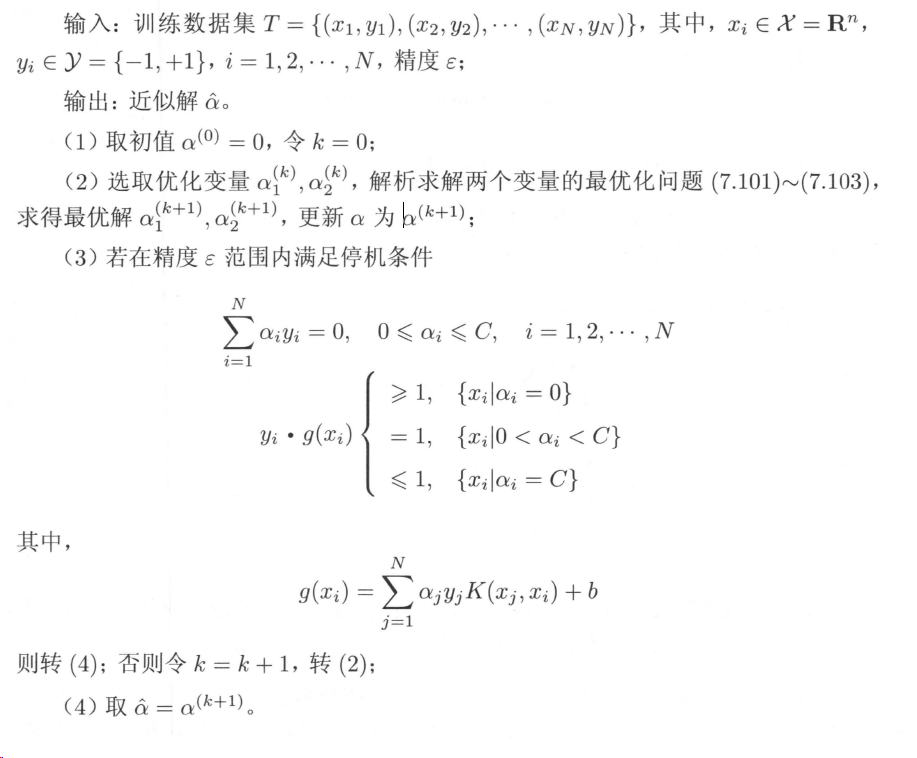
\includegraphics[width=0.7\linewidth]{screenshot002}
	\label{fig:screenshot002}
\end{figure}

\section{实验步骤}
\subsection{数据集来源}
本次实验采用来自MNIST数据集(Mixed National Institute of Standards and Technology database),美国国家标准与技术研究院收集整理的大型手写数字数据库,包含60,000个示例的训练集以及10,000个示例的测试集
\subsection{数据加载}
利用torchvision中所集成的MNIST数据集加载数据,此时返回的数据为PIL Image格式,在后续处理中,直接利用$numpy.array()$将其转化为数组处理即可。
\lstinputlisting[language=Python]{./code/1.txt}
\subsection{SVM算法训练}
在训练过程中,将数据分batch依次加载到模型中,如此可提高算法的训练速度和训练精度。SVM.py实现了一个SVM多分类器,具体实现原理是:对于样本中的每两个类别之间都训练一个SVM二分类器。对于$k$个类别,共可训练出$k(k-1)/2$个SVM二分类器。在预测时,将测试样例分别输入到$k(k-1)/2$分类器中。假设$(i,j)$表示划分类别$i$和类别$j$的SVM分类器,对于每个分类器$(i,j)$:
\begin{itemize}
	\item 若分类结果为$+1$,则$count[i] +=1$
	\item 若分类结果为$-1$,则$count[j] +=1$
\end{itemize}
最后分类结果取相应类别计数最大的那个类别作为最终分类结果。SV.py还实现了将训练的模型保存成文件,方便预测时直接从文件读取,省去了再次训练的时间。训练求解过程中采用SMO进行优化,在选择优化变量时,选择误差步长最大的两个变量进行优化,如此可以大幅提高优化速度。同时采用了RBF核函数,具体实现参见$kernelTrans(self,x,z)$。详细代码见附录或\url{https://github.com/ZS-Yan/SVM-digit-recognition}.

最终在MNIST数据集上得到了92.48\%的准确率。

\section{实验分析}
SVM作为经典的分类器模型,在手写数字识别任务依然取得了不错的准确率。且相较于现代神经网络方法,能够保持参数量低的优势同时取得较高准确率。理解SVM无论是对数学基础或是编程能力均是一次极大的考验,在此向提出这些经典且精妙的大师们致敬!

%\begin{table}[H]
%	\renewcommand{\arraystretch}{1.0}
%	\centering
%	\caption{\centering 固定优化器和惩罚项调整多分类处理方式}
%	\begin{threeparttable}
%		\begin{tabular}{lll}
%			\toprule[1.5pt]
%	         & ovr & multinomial \\
%			\midrule[1pt]
%			Accuracy &   91.1977\%  & \textbf{98.5845}\%    \\
%			Recall   &  91.3801\%   & \textbf{95.3188}\%  \\
%			\bottomrule[1.5pt]
%		\end{tabular}
%		\begin{tablenotes}
%			\footnotesize
%			\item[1] 设置solver='saga'
%			\item[2] 设定penalty='elasticnet'
%		\end{tablenotes}
%	\end{threeparttable}
%\end{table}

\section{参考文献}
\begin{enumerate}[itemsep=0.01pt]
	\item[] [1] 周志华. 机器学习[M]. 清华大学出版社, 2016.
	\item[] [2] 李航. 统计学习方法[M]. 清华大学出版社, 2019
	\item[] [3] https://zhuanlan.zhihu.com/p/31886934 
	\item[] [4] Christopher M. Bishop: Pattern Recognition and Machine Learning, Chapter 4.3.4
\end{enumerate}




%\newpage
%\begin{center}
%	\Large{\textbf{\heiti 附录}}
%\end{center}

%\appendix
% \renewcommand{\appendixname}{Appendix~\Alph{section}}

%\section{附录1 -- 程序流程框图}
%
%\begin{figure}[H]
%	\centering
%	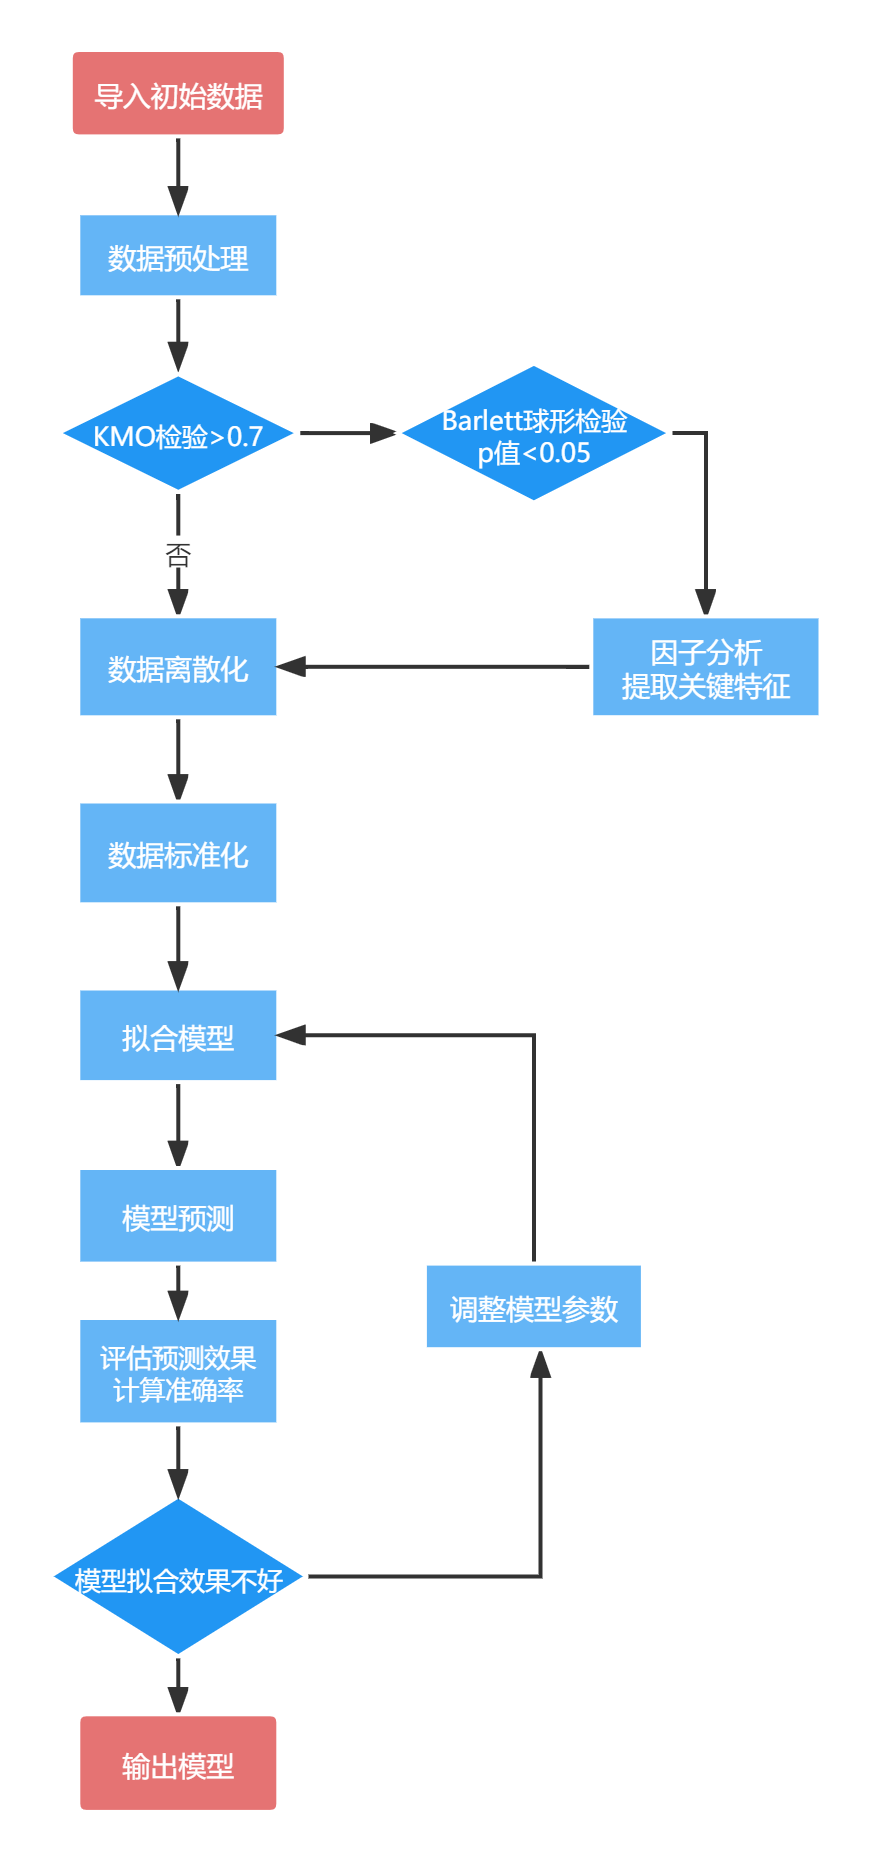
\includegraphics[width=0.6\textwidth]{流程图.png}
%	\caption{\centering  程序流程框图}
%\end{figure}

\section{附录 -- SVM实验完整代码 }
SVM.py
\lstinputlisting[language=Python]{./code/2.txt}
\newpage
SMO.py
\lstinputlisting[language=Python]{./code/3.txt}
\end{document}